\documentclass[12pt,a4paper]{article}
\usepackage[spanish,es-tabla]{babel}
\usepackage{bbm}
\usepackage[utf8]{inputenc}
\usepackage{multicol}
\usepackage[T1]{fontenc}
\usepackage{graphicx}
\usepackage{gensymb}
\usepackage{amssymb, amsmath} %Paquetes matemáticos de la American Mathematical Society
\parskip=1 mm
\oddsidemargin -0.8 cm
\headsep -2 cm
\textwidth=17.8cm
\textheight=25.5cm
\begin{document}
\title{Laboratorio de Mecánica, Práctica 7 - Péndulo Simple}
\date{26 de marzo del 2025}
\author{\textbf{Ortega Montero Fernando Naed} - Equipo 4\\
Yibran Morales Munguía\\
Victor Manuel Santillan Romero}
\maketitle
\section{Resumen} 

En este informe se expone el experimento de un péndulo simple bajo ángulos pequeños; midiendo el cambio en el periodo de el péndulo dependiendo de la longitud de la cuerda, esto con el objetivo de encontrar la constante de aceleración gravitacional ($g$) y medir el error comparado con el valor convencionalmente verdadero para la altura de la Ciudad de México. 

\section{Introducción}

El péndulo simple es un sistema que consta de una masa que puede oscilar colgada de un punto, para este informe se usará el modelo ideal del péndulo simple, por lo que se considerará una cuerda sin masa, inextensible, con ángulos de oscilación muy pequeños, sin velocidad inicial aplicada sobre la masa y sin fricción del aire.\\
Con esto podemos plantear una ecuación que describa el periodo de un péndulo simple que solo dependa de la longitud.\\

\[T = \frac{2\pi}{\sqrt{g}} \ell^{\frac{1}{2}}\]

En esta ecuación se hará un cambio de variable de $L = \ell^{\frac{1}{2}}$ con el objetivo de obtener una ecuación de primer grado, donde esta quedará como: 

\[T = \frac{2\pi}{\sqrt{g}} L\]

Nótese que en esta ecuación la pendiente será… 

\[m = \frac{2\pi}{\sqrt{g}}\]

Por lo que despejando $g$ tendremos que…

\[g = \frac{4\pi^2}{m^2}\]

Como valor convencionalmente verdadero se tomará:

\[g = 9.78 \frac{m}{s^2}\]

Esto pensando en el valor para la altura de la Ciudad de México. 

\section{Desarrollo experimental}

Para la práctica se utilizó un soporte universal, dos varillas, una nuez, un flexómetro (con resolución de 0.001 m), una plomada, un hilo de 4 m y un cronometro (con una resolución de 0.01 s).\\
Se colocó el soporte universal en una mesa, se colocó una de las varillas en vertical con ayuda del soporte universal, se colocó la segunda varilla en perpendicular a la primera varilla con ayuda de la nuez. \\
A la varilla horizontal se sujetó el hilo en forma de “v” (atando la cuerda en dos puntos de la varilla y dejando un pedazo de cuerda que una estas dos ataduras, de en medio de este pedazo de cuerda se colocará la plomada, que fungirá como la masa del péndulo) para evitar el movimiento fuera del eje de medición. \\
La longitud tomada será perpendicular a la varilla y será la distancia entre la varilla y la plomada (nótese que no se tomará en cuenta la longitud de la cuerda entre le varilla y la plomada).\\

Se soltará la plomada con la cuerda tensa con un ángulo pequeño y se medirá el tiempo de diez oscilaciones, este tiempo se tomará cinco veces para cada longitud de la cuerda, a pesar de que el ángulo y el periodo cambie con cada oscilación este cambio es despreciable por lo que solo se dividirá el tiempo obtenido entre 10 para obtener el periodo de una oscilación. \\

\section{Resultados}

En la Tabla 1 se exponen los promedios de cinco mediciones después de haber encontrado el promedio de una solo oscilación, las distancias y la variable $L = \ell^{\frac{1}{2}}$ esta variable servirá debido a que la función $T(\ell)$ no es una ecuación lineal por lo que se hace el cambio de variable $T(L)$ para que la ecuación sea lineal y se pueda hacer la debida regresión lineal, todo esto con el objetivo de calcular finalmente la constante gravitacional ($g$)

\subsection{Calculo de la incertidumbre}

Para el cálculo de incertidumbre estándar combinada del periodo se hará uso de la siguiente ecuación:

\[u_c(T) = \sqrt{u_A^2(T) + u_B^2(T)}\]

Donde…\\

$u_c(T)$ : Es la incertidumbre estándar combinada del periodo.\\

$u_A(T)$ : Es la desviación estándar de la media de los tiempos medidos en cada longitud \\

$u_B(t)$ : Es la incertidumbre del cronometro (Su precisión).\\

Nótese que este cálculo se hizo para el promedio de los tiempos en cada longitud, así mismo nótese que no se usara la precisión del cronometro como la incertidumbre tipo B, sino el promedio de los mínimos tiempos posibles medidos por uno de los experimentadores autores de este informe, este promedio fue 0.16 s, este tiempo será tomado como la incertidumbre tipo B.\\

De esto sigue la propagación de la incertidumbre para la variable  $L = \ell^{\frac{1}{2}}$, usando la ley de la propagación de la incertidumbre tenemos la siguiente ecuación:

\[u^2_c (L) = \sum_{i = 1}^k \left( \frac{\partial L}{\partial x_i}\right) u^2(x_i)\]

Donde…\\

$u^2_c(L)$ : Es la incertidumbre de la variable L.\\

$x_i$ : Son las variables de las cuales depende la variable L; $L(x_1, x_2, …, x_k)$. Nótese que la variable L solo depende de $\ell$; $L(\ell) = \ell^{\frac{1}{2}}$, por lo que $x_i = \ell$.\\

$k$ : Son el número de variables de las cuales depende la variable L. Nótese que la variable L solo depende de $\ell$, por lo que $k = 1$.\\

$u^2(x_i)$ : Es la incertidumbre de cada variable de las cuales depende la variable L. Nótese que la variable L solo depende de $\ell$, por lo que $u^2(x_i) = u^2(\ell)$.\\

$\frac{\partial L}{\partial x_i}$: Es la derivada parcial de cada variable de las cuales depende la variable L. Nótese que la variable L solo depende de $\ell$, por lo que $\frac{\partial L}{\partial x_i} = \frac{d L}{d \ell} = \frac{1}{2\sqrt{\ell}}$.\\

Finalmente, esta ecuación nos queda:

\[u^2_c (L) = \sum_{i = 1}^1 \left( \frac{\partial L}{\partial \ell}\right)^2 u^2(\ell)\]
\[u^2_c (L) =\left(\frac{1}{2\sqrt{\ell}}\right)^2 u^2(\ell)\]
\[u_c (L) = \frac{1}{2\sqrt{\ell}} u(\ell)\]

Nótese que este calculo se hizo para cada $\ell$. Ademas nótese que la incertidumbre de $\ell$ es igual a la precisión del felxometro, $u(\ell) = 0.001 m$ 



\begin{table}[h!]
\begin{center}
\begin{tabular}{|c|c|c|c|}
\hline
No. & T (s) & $\ell$ (m) & $L = \ell^{\frac{1}{2}}$ ($m^{\frac{1}{2}}$)\\
\hline
1 & 2.04 (0.16) s & 1.000 (0.001) m & 1.000 (0.001) $m^{\frac{1}{2}}$ \\ \hline
2 & 2.10 (0.16) s & 1.074 (0.001) m & 1.024 (0.001) $m^{\frac{1}{2}}$ \\ \hline
3 & 2.27 (0.16) s & 1.200 (0.001) m & 1.063 (0.001) $m^{\frac{1}{2}}$ \\ \hline
4 & 2.34 (0.16) s & 1.351 (0.001) m & 1.105 (0.001) $m^{\frac{1}{2}}$ \\ \hline
5 & 2.42 (0.16) s & 1.400 (0.001) m & 1.119 (0.001) $m^{\frac{1}{2}}$ \\ \hline
6 & 2.48 (0.16) s & 1.562 (0.001) m & 1.160 (0.001) $m^{\frac{1}{2}}$ \\ \hline
7 & 2.53 (0.16) s & 1.582 (0.001) m & 1.165 (0.001) $m^{\frac{1}{2}}$ \\ \hline
8 & 2.65 (0.16) s & 1.600 (0.001) m & 1.170 (0.001) $m^{\frac{1}{2}}$ \\ \hline
9 & 2.70 (0.16) s & 1.800 (0.001) m & 1.216 (0.001) $m^{\frac{1}{2}}$ \\ \hline
10 & 2.96 (0.16) s & 1.950 (0.001) m & 1.249 (0.001) $m^{\frac{1}{2}}$ \\ \hline
\end{tabular}
\caption{Periodos medidos por una oscilación de un pendulo en función de la longitud}
\end{center}

\end{table}
\begin{figure}[h!]
\centering
\includegraphics[scale=0.58]{2.png}
\caption{Grafica de los $\ell$ - T}
\end{figure}

\begin{figure}[h!]
\centering
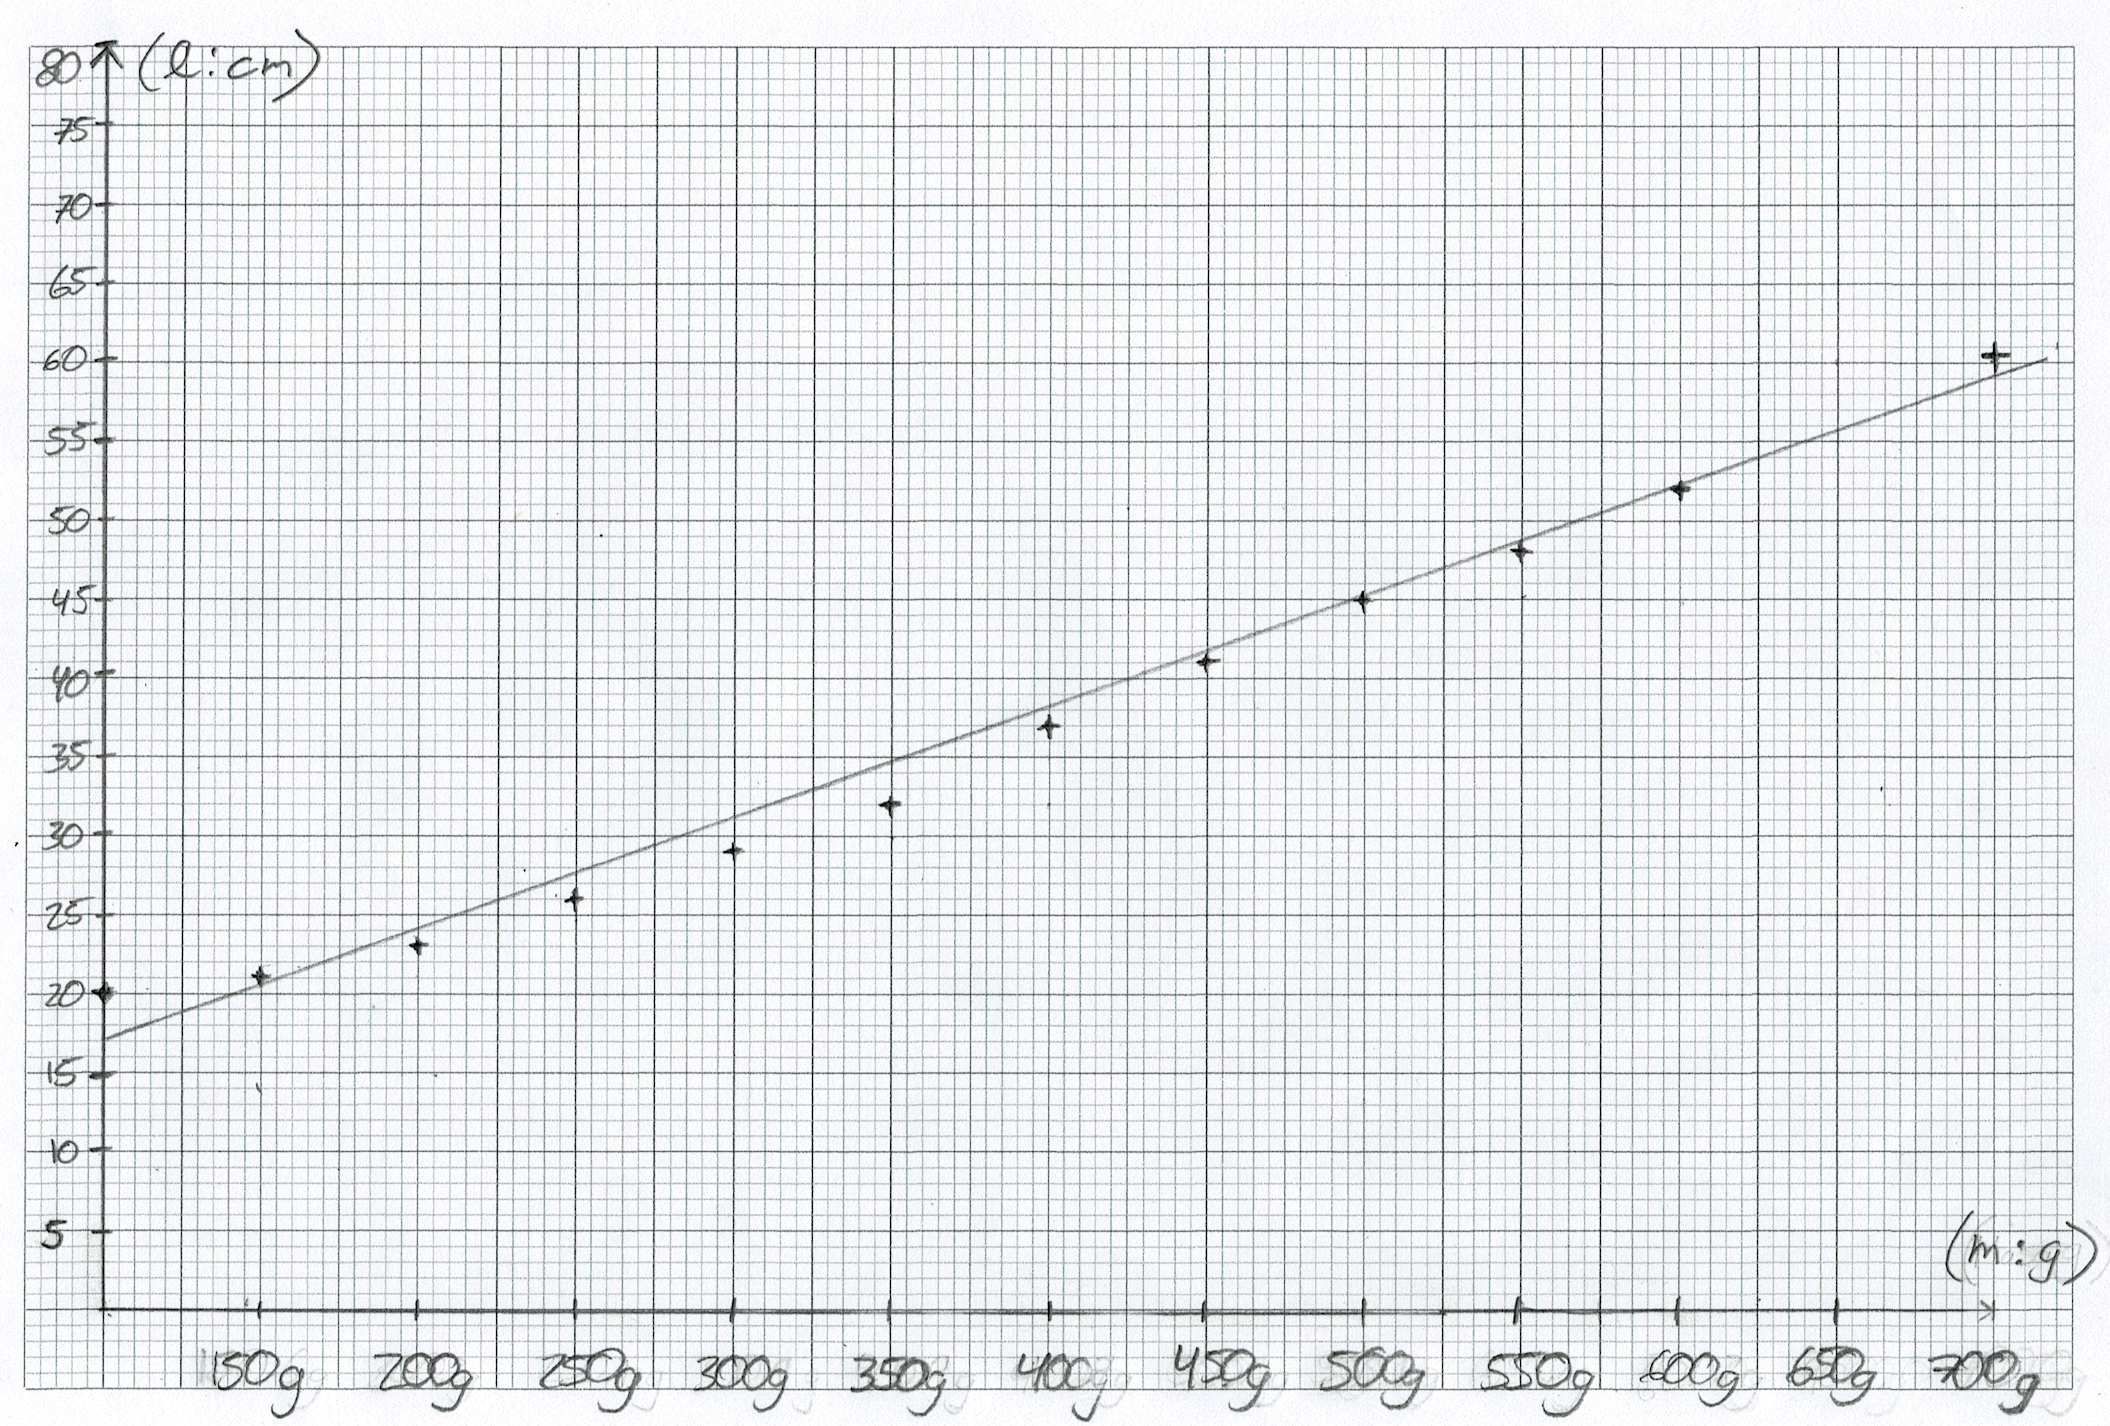
\includegraphics[scale=0.58]{1.png}
\caption{Grafica de los $\ell^{\frac{1}{2}}$ - T}
\end{figure}

\newpage

\section{Discusión}

Nótese finalmente que al ocupar la ecuación que nos da la constante de aceleración de la gravedad tenemos que 

\[g = \frac{4\pi^2}{m^2} = 8.44\]

De lo cual se obtendrá el error tomando en cuenta el valor convencionalmente verdadero.

\[\varepsilon = |9.78 – 8.44| = 1.34\]

El resultado se desvía bastante del del valor convencionalmente verdadero. 

\section{Conclusión}

Se encuentra que el valor medido experimentalmente se aleja bastante del valor convencionalmente verdadero; al escribir este informe me di cuenta de la pobre organización de mis datos experimentales, encontrando algunos datos sin ningún tipo de sentido escritos en mi bitácora. Por lo que puedo discernir que a pesar de que la práctica se haya realizado con éxito en el laboratorio, no se logro concluir correctamente en este informe.  


\section{Referencias}

Miranda, Javier. (2025) \textit{Física Experimental. Introducción a los conceptos y métodos.} Recuperado el 18, 03, 2025, de https://copitarxives.fisica.unam.mx/LT0006ES/LT0006ES.pdf \\

Miranda, Javier. (2000). \textit{EVALUACIÓN DE LA INCERTIDUMBRE EN DATOS EXPERIMENTALES.} \\

Pérez, Héctor. (2018). \textit{Física general.}(Sexta Edición.). México: PATRIA educación \\

Alonso, V. (2018). \textit{Péndulo simple.}



\end{document}